\chapter{System Development}

\section{Design}

System design is covered here with the intent of allowing for future modification or reproduction of the flow system. Development of neither the labVIEW Virtual Interface (VI) nor microcontroller are covered in detail but are presented in the attached appendixes. The electronics skills required to build the system include analogue and digital electronics but are of basic undergraduate level and are not covered in any detail here. 

\qquad


\paragraph{Design Inputs} High level design inputs were generated by discussion with the the research group of Thomas Franke and may be summarized as follows:


\begin{enumerate}
\item The flow system shall be controlled by a labVIEW VI.
\item The flow system shall feature four discrete pressure channels.
\item The flow system shall be capable of producing pressure output 
from 0 to 1 bar.
\item The resulting controlled pressure shall be visible to and recordable by the user.
\end{enumerate}

\clearpage

\paragraph{System Components}In order to develop a system capable of meeting these design inputs several key components are required, specified in Table \vref{tab:syscomp}

\qquad

 
\begin{table}[H]
\begin{center}
\begin{tabular}{l*{6}{c}r}
Component & Manufacturer & Part Number & Quantity \\
\hline
Regulators & Marsh Bellofram & Type 2000 & 4 \\
Transducers & AMS & 5915-1000-D & 4\\
Transducers & AMS & 5915-0350-D & 4\\
DACs & MCP & 4921 & 4\\
Microcontroller & Arduino & Uno R3 & 1 \\
\end{tabular}
\caption [Key System Components]{Key System Components} 
\label{tab:syscomp}
\end{center}
\end{table}

Alternative components may be acceptable, even superior, to those detailed here. Specifically, pressure transducers that allow for faster modulation may be sought. The time response of the system developed here is covered in Section \ref{sec:characterization}. In addition to the key components listed here other basic electrical components were required including standard off-the-shelf resistors, capacitors, molex-connectors and prototyping solderboard.

The system electronics are packaged within a IP 66/IP 67 DIN EN 60529 rated enclosure, shown in Figure \vref{fig:sysPhoto}. The system functions as a 'black box' with the 240VAC$->$9VDC power input, USB communication, main pneumatic supply line input, and 4 discrete regulated pressure outputs.

\begin{figure}[H]
\centering 
\includegraphics[width=0.750\columnwidth]{sysPhoto.PNG} 
\caption[Image of Packaged PDFC]{The PDFC as contained in the final enclosure.} 
\label{fig:sysPhoto} 
\end{figure}

Several pneumatic components are required to provide a compressed gas flow path between the supply, the regulators, transducers, and reagent reservoirs. These components are summarized in the pneumatic schematic for a single channel is shown in Figure \vref{fig:pneumaticSchematic}. Note that the air supply here is expected to be filtered to remove excess humidity and provide 3 micron particle filtration. 

\begin{figure}[H]
\centering 
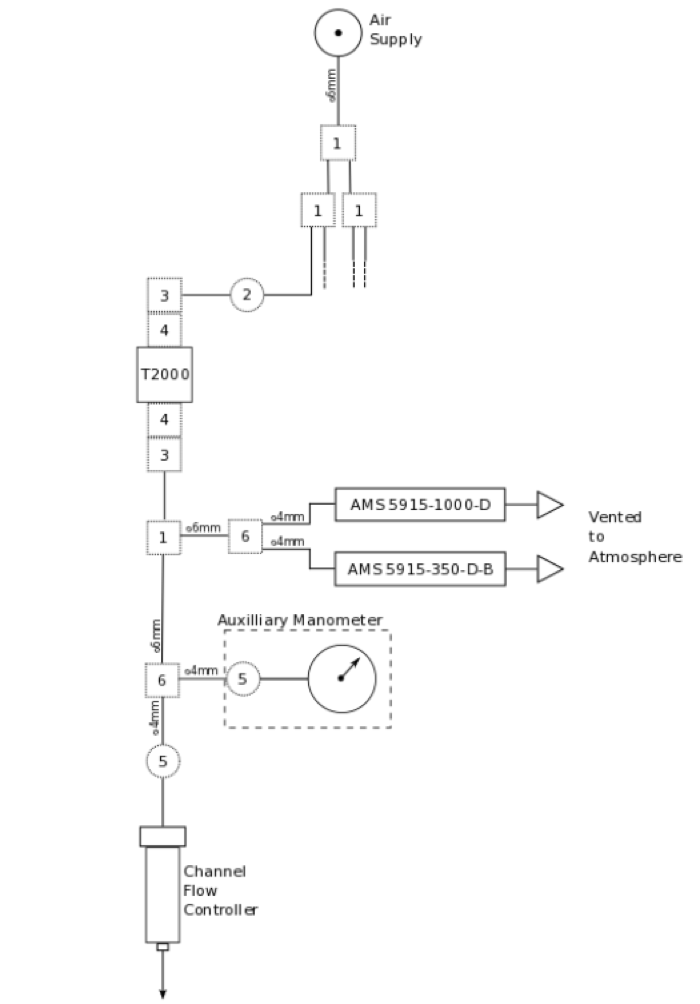
\includegraphics[width=1.0\columnwidth]{pneumaticSchematic.PNG} 
\caption[Pneumatic Schematic of PDFC channel]{The pneumatic schematic detailing a single channel of the PDFC. The four primary components moving down through the schematic are the supply, T2000 pressure regulator, AMS pressure transducers, and the terminal flow reservoir.} 
\label{fig:pneumaticSchematic} 
\end{figure}

\paragraph{Operational Overview} The PDFC system is designed to be managed by interaction with a custom LabVIEW VI. The user manually enters a desired control signal within the labVIEW interface of 0 to 5 volts, corresponding to operational pressure range of 0 to 1000mbar.

\begin{figure}[H]
\centering 
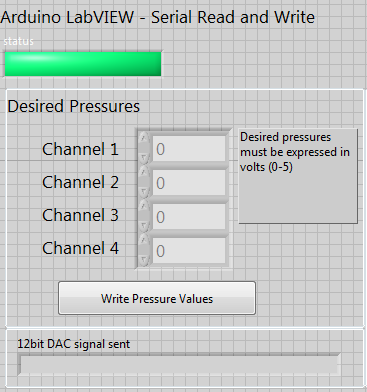
\includegraphics[width=0.5\columnwidth]{writeVI.PNG} 
\caption[LabVIEW write command]{Control pressures are set digitally within the LabVIEW interface.} 
\label{fig:writeVI} 
\end{figure}

After initiating the write command the digital signal is written synchronously to the micro-controller by Universal Serial Bus (USB) via LabVIEW's 'virtual instrument software architecture'. The signal is initially sent and interpreted as a string and is processed via the embedded micro-controller code into a binary command comprised of the 4 configuration bits and 12 data bits. This binary command is then written to the digital analogue converters (DACs) via standard serial peripheral  interface (SPI) protocol. The DACs convert the binary commands into analogue voltage outputs of 0-5V. This voltage is routed to the input of each pressure regulator and results in the desired pressure output of 0 to 1000 mbar.

The controlled output of each pressure regulator is then split by a y-connector. One flow path goes to the reagent reservoir to drive fluid flow, the other is routed back into the PDFC for real-time measurement by the integrated chip pressure transducers. Each regulated pressure channel is measured by two different 14bit transducers, one is low range (0-350mbar) with increased resolution, the other is full range (0-1000mbar). The pressure transducers produce a digital signal that is then transferred back to the micro-controller via I2C protocol. Finally the measured pressures are sent to the LabVIEW VI for display and optional recording. This entire control process including LabVIEW and microfluidic device integration is summarized in system overview shown in Figure \vref{fig:systemOverview}.



\begin{figure}[H]
\centering 
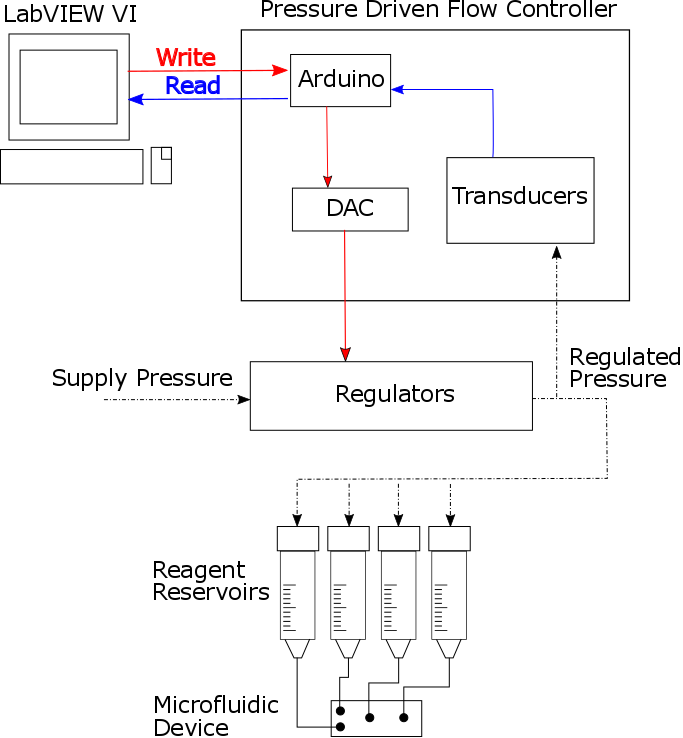
\includegraphics[width=1.0\columnwidth]{systemOverview.PNG} 
\caption[System Overview of the PDFC]{The control loop used to set and measure channel pressures using the PDFC} 
\label{fig:systemOverview} 
\end{figure}

\clearpage

\section{Characterization}
\label{sec:characterization}


After completing manufacture and integration of the PDFC it must be validated prior to being used as a research tool. Particular emphasis is placed on two operating criteria of the system:
\begin{enumerate}
\item The response time of the system, from application of write signal to regulated pressure response.
\item The accuracy and channel-to-channel variance observed in the system.
\end{enumerate}

In regards to the response time of the system it may be valuable to detail the magnitude of individual response times for the process steps required from signal input to response output, summarized in Table \vref{tab:compTime}

\begin{table}[H]
\begin{center}
\begin{tabular}{l*{6}{c}r}
Process Step & Magnitude of Time Response(ms) \\
\hline
Sync. USB Comm. & 1000 \\
Arduino String $->$ Binary & 1 \\
DAC & 1\\
Pressure Regulator & 100\\
\end{tabular}
\caption [Component Response Time]{Component Response Time} 
\label{tab:compTime}
\end{center}
\end{table}

The labVIEW VI is capable of recording the measured regulated pressure outputs, which may be used to document control pressures utilized for specific experimentation. Here, that data logging capability is used to investigate the system's time response, as shown in Figure \vref{fig:timeResponse}. The gap in data is due to use of 'synchronous' USB communication within the LabVIEW environment. The rightmost data prior to the gap coincides with the time point at which the command signal is sent. While all channel outputs clearly converge to the desired nominal output pressure, the time response is broadly speaking slow, and variation in channel regulation is apparent as the pressure output stabilizes. Variation in the stabilization of regulated signal is due to differences in the control circuit from regulator to regulator. The model of regulator used here relies on a Proportional Integral Differential (PID) control circuit with manually adjustable potentiometers to adjust gain constants, non-ideal when attempting to produce coincident outputs on discrete channels.

The time from signal write to that of reaching $95\%$ of the desired output, $\tau$, increases as a function of differential pressure sought but is roughly on the magnitude of $~1 sec$. 

\begin{figure}[H]
\centering 
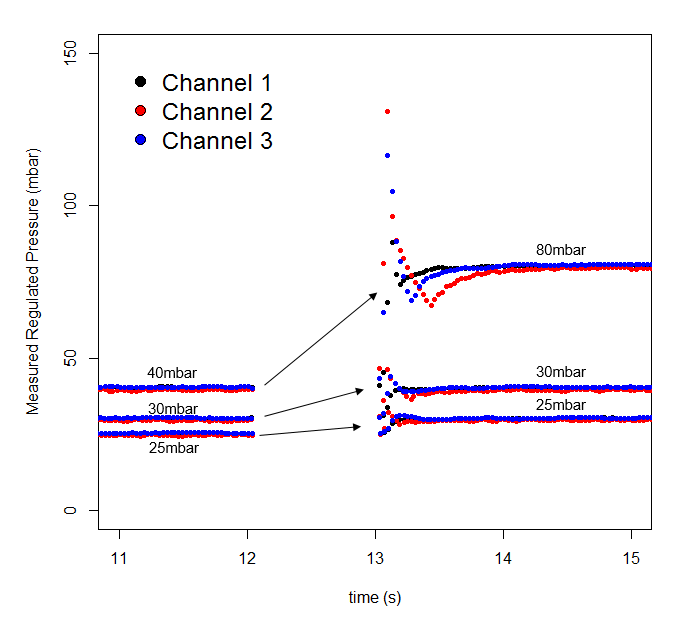
\includegraphics[width=01.0\columnwidth]{timeResponse.PNG} 
\caption[PDFC time response]{Three pressure transitions are shown, 40 to 80mbar, 30 to 40mbar, and 25 to 30mbar for 3 discrete output channels. } 
\label{fig:timeResponse} 
\end{figure}

These observations suggests that the system, as currently developed, is not appropriate for the millisecond or faster response times required for real-time manipulation of droplet size. This agrees with previous findings. Flow rate control of droplet formation is known for its slow response whether by syringe pump or pressure flow. Furthermore, response time of the actual device is further delayed due to fluidic capacitance caused by the compressibility of reagents, tubing and PDMS channels \cite{Churski2013,Stone2004}. If fast-response times are sought a more appropriate methodology may be to maintain a steady flowrate and drive droplet formation by active methods through direct manipulation of the fluid at the local point of formation by electrical, mechanical, magnetic, or acoustic means \cite{Chong2016}.


System accuracy and channel to channel variation can be investigated in a similar method to time response. Here, three channels are simultaneously regulated to a nominal 100mbar. After a stabilization time of approximately 3 seconds, a 15 second mean and standard deviation are acquired for each channel, as shown in area between the dashed lines in Figure \vref{fig:constV}. Each channel is capable of regulating to the nominal 100 $\pm$ 1 mbar with a standard deviation of less than 0.25 mbar. The capability to maintain stable pressure and hence steady flow is critical for production of highly monodispersed droplets, as documented in Results section \ref{sec:results}.


\begin{figure}[H]
\centering 
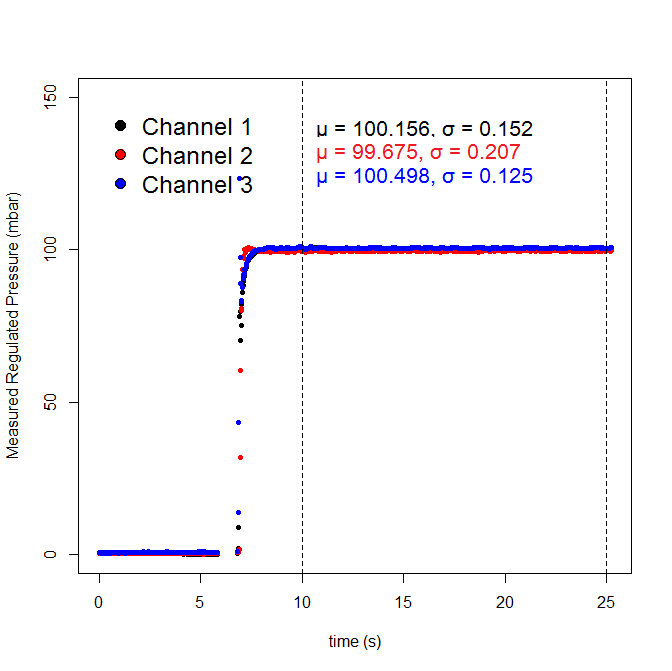
\includegraphics[width=01.0\columnwidth]{constV.PNG} 
\caption[PDFC accuracy and inter-channel variation]{Accuracy and channel-to-channel variation of the PDFC system.} 
\label{fig:constV} 
\end{figure}